\documentclass{article}

% Packages
\usepackage[utf8]{inputenc} % For modern characters
%\usepackage{microtype} % For sexy kerning
\usepackage{mathtools} % For math stuff
\usepackage{amssymb} % For math symbols
\usepackage{tabularx} % For making tables
\usepackage{listings} % For writing code
\usepackage{fancyhdr}
\usepackage{pdfpages}


% Other front matter
\lstset{language=R} % Set listing language to R
\newcommand{\tab}{\hspace*{3em}} % 
\pagestyle{fancy}
\lhead{}
\chead{}
\rhead{Ben Foster | Homework 1 | April 7, 2015}
\setcounter{tocdepth}{2}

\begin{document}

% Title page, table of contents, and page number setting
{
	\title{Probability and Statistics for Engineers Homework One \\ TMATH 390}
	\author{Ben Foster\thanks{
		Institute of Technology, University of Washington Tacoma} \\
		Instructor: Julia Eaton }
	\date{April 7, 2015}
	\maketitle
	\thispagestyle{empty} % Gets rid of the page number at the bottom
	\clearpage
	
	
	\pagenumbering{roman}
	\tableofcontents
	\clearpage
	\setcounter{page}{1}
	\pagenumbering{arabic}
}

\section*{Problem 1}
\addcontentsline{toc}{section}{First Problem}

	Collect data according to the following specifications. Most sources are allowed: web, books,
	papers, your own work, etc. but do not use the preloaded data that comes with R. \\
	
	\noindent Specifications:
	\begin{itemize}
		\item{Number of cases: 10 or more.}
		\item{2 categorical or discrete variables.}
		\item{2 continuous quantitative variables.}
		\item{These 4 variables must relate to a common problem; do not give me 4 unrelated
		variables.}
	\end{itemize}
	
	\noindent Turn in a print out of the data. We will use this data in future problems.
	
	\begin{table}[!htb]
	\begin{tabular}{ | c || c | c | c | c | } \hline
		Artist & Genre & Gender & Avg. length of song & Avg. $\frac{words}{song}$ \\ \hline \hline
		Jimi Hendrix & Classic Rock & Male & 7.35 min & 189.4 \\ \hline % 1
		Madonna & Pop & Female & 5.22 min & 120.2 \\ \hline % 2
		Skrillex & Dubstep & Male & 4.45 min & 13.7 \\ \hline % 3
		Eminem & Rap & Male & 6.14 min & 428.38 \\ \hline % 4
		Aesop Rock & Rap & Male & 7.78 min & 932.2 \\ \hline % 5
		Sia & Pop/Rock & Female & 4.69 min & 279.9 \\ \hline % 6
		Lorde & Pop & Female & 3.58 min & 155.01 \\ \hline % 7 
		Beck & Alt Rock & Male & 4.57 min & 180.34 \\ \hline % 8
		R. Kelly & R\&B & Male & 4.38 min & 210.23 \\ \hline % 9
		James Brown & R\&B & Male & 5.27 & 280.56 \\ \hline % 10
	\end{tabular}
	\caption{Solo Artists}
	\label{tab:solo_artists}
	\end{table}

\clearpage
\section*{Problem 2}
\addcontentsline{toc}{section}{Second Problem}

	Temperature transducers of a certain type are shipped in batches of 50 units. A sample of 60
	batches was selected, and the number of transducers in each batch not conforming to design
	specifications was determined, resulting in the following data:
	
	\vspace{-1.0\baselineskip}
	\begin{table}[!htb]
	\begin{tabular}{ c c c c c c c c c c c c c c c c c c c c }
		2 & 1 & 2 & 4 & 0 & 1 & 3 & 2 & 0 & 5 & 3 & 3 & 1 & 3 & 2 & 4 & 7 & 0 & 2 & 3 \\
		0 & 4 & 2 & 1 & 3 & 1 & 1 & 3 & 4 & 1 & 2 & 3 & 2 & 2 & 8 & 4 & 5 & 1 & 3 & 1 \\
		5 & 0 & 2 & 3 & 2 & 1 & 0 & 6 & 4 & 2 & 1 & 6 & 0 & 3 & 3 & 3 & 6 & 1 & 2 & 3 \\
	\end{tabular}
	\end{table}
	\vspace{-1.0\baselineskip}
	
	\noindent (a) Determine the frequencies and relative frequencies for the observed values of x, 
	which is the number of nonconforming transducers in a batch. \\
	\noindent (b) What proportion of batches in the sample have at most five nonconforming 
	transducers?
	%\vspace{-1.0\baselineskip}
	
	\paragraph{Answer to a} 
	There is a way in R to input data and get the frequencies of each. To do so by hand, you would 
	count each time the specific number showed up in the data presented and keep a running count 
	which would be the "frequency" of each. To find the "relative frequency" of each, you would 
	divide each of the frequencies by the total number of data in the sample. Here is the code you 
	would type in R to figure out the answers the easy way:
	
	\begin{lstlisting}[frame=single]
    > data <- c(2,1,2,4,0,1,3,2,0,5,3,3,1,3,2,4,7,0,2,
    3,0,4,2,1,3,1,1,3,4,1,2,3,2,2,8,4,5,1,3,1,5,0,2,3,
    2,1,0,6,4,2,1,6,0,3,3,3,6,1,2,3)

    > table(data)

    > table(data) / length(data)
	\end{lstlisting} 
	
	\noindent Here is the table of Frequency and Relative Frequency that came from R: 

	\begin{table}[!htb]
	\centering
	\begin{tabular}{ | c | c | c | }
		\hline
		\textbf{Value} & \textbf{Freq} & \textbf{Relative Freq.} \\ \hline \hline
		0 & 7 & 0.11667 \\ \hline
		1 & 12 & 0.20 \\ \hline
		2 & 13 & 0.21667 \\ \hline
		3 & 14 & 0.23333 \\ \hline
		4 & 6 & 0.10 \\ \hline
		5 & 3 & 0.050 \\ \hline
		6 & 3 & 0.050 \\ \hline
		7 & 1 & 0.01667 \\ \hline
		8 & 1 & 0.01667 \\ \hline
	\end{tabular}
	\label{tab:frequency_table}
	\end{table}
	\vspace{-1.0\baselineskip}
	
	\paragraph{Answer to b}
	To do this problem by hand, you would have to take the relative frequencies of all the values 
	less than or equal to five and add them together. To do this in R, you just have to type the 
	command \texttt{> sum(data <= 5) / length(data)} and that will give you the answer which is 
	0.91667.

\section*{Problem 3}
\addcontentsline{toc}{section}{Third Problem}

	A continuous variable x is said to have a \textit{uniform} distribution if the density function is 
	given by
	
	\begin{displaymath}
		f(x) = \left\{
			\begin{array}{lr}
				\frac{1}{b - a}, & $if $ a < x < b \\
				0, & otherwise.
			\end{array}
		\right.
	\end{displaymath}
	
	\noindent The corresponding density "curve" has constant height over the interval from $a$ to 
	$b$. Suppose the time taken by a clerk to process a certain application form has a uniform 
	distribution with $a = 4$ minutes and $b = 6$ minutes. \\
	
	\noindent (a) Verify that the total area under the curve is indeed 1. \\
	(b) In the long run, what proportion of forms will take between 4.5 min and 5.5 min to 
	process? \\
	(c) What value separates the slowest 50\% of all processing times from the fastest 50\% (the
	median of the distribution)? \\
	(d) What value separates the fastest 10\% of all processing times from the remaining 90\%?
	
	\paragraph{Answer to a} In order to answer question a by hand, you would have to take the 
	integral of the function from $a$ to $b$ with respect to $x$ and the answer had to be equal to 
	one. In this case, $a = 4$ and $b = 6$ which makes it a little easier to answer. In R, all you have 
	to do is define the function and then integrate it. Here is the code to do that:
	
	\begin{lstlisting}[frame=single]
    # Define the function as well as a and b
    > fx <- function(x) \{ifelse(x > a & x < b,
    1 / (b - a), 0)\}
    > a = 4
    > b = 6
    
    # Integrate the function
    > integrate(fx, a, b)
	\end{lstlisting}
	
	\noindent The answer you would get from this is 1. Thus verifying the total area under the curve.
	\\ \\
	\noindent Here's how to do it by hand:
	\begin{displaymath}
		\int_{a}^{b} \frac{1}{b - a} dx \\
		= \int_{4}^{6} \frac{1}{6 - 4} dx \\
		= \frac{1}{2} \int_{4}^{6} 1 dx \\
		= \frac{1}{2} \left[ 6 - 4 \right] \\
		= 1
	\end{displaymath}
	\clearpage
	
	\paragraph{Answer to b}
	To answer this question using R, you would keep the same function that was defined as above 
	and you would also use the integrate() function, however you would replace $a$ with 4.5 and 
	$b$ with 5.5 like so: \texttt{> integrate(fx, 4.5, 5.5)} \\ \\
	Here's how to do it by hand:
	
	\begin{displaymath}
		\int_{4.5}^{5.5} \frac{1}{6 - 4} dx \\
		= \frac{1}{2} \int_{4.5}^{5.5} 1 dx \\
		= \frac{1}{2} \left[5.5 - 4.5 \right] \\
		= 0.5
	\end{displaymath}
	
	\paragraph{Answer to c}
	Since it is easier to just answer this question by hand, then that is how I will do it. We have to 
	find the value $b$ such that $\int_{4}{b} \frac{1}{6 - 4} dx = 0.5$.
	
	\begin{displaymath}
		\int_{4}^{b} \frac{1}{6 - 4} dx \\
		= \frac{1}{2} \int_{4}^{b} 1 dx \\
		= \frac{1}{2} \left[b - 4 \right]
	\end{displaymath}
	\begin{displaymath}
		\frac{1}{2} \left[b - 4 \right] = 0.5
	\end{displaymath}
	\begin{displaymath}
		b - 4 = 1
	\end{displaymath}
	\begin{displaymath}
		b = 5
	\end{displaymath}
	
	\paragraph{Answer to d}
	The process of figuring out the answer to this problem is very similar to the last one. All we have 
	to do in this case is find the value $b$ such that $\int_{4}{b} \frac{1}{6 - 4} dx = 0.1$.
	
	\begin{displaymath}
		\int_{4}^{b} \frac{1}{6 - 4} dx \\
		= \frac{1}{2} \int_{4}^{b} 1 dx \\
		= \frac{1}{2} \left[b - 4 \right]
	\end{displaymath}
	\begin{displaymath}
		\frac{1}{2} \left[b - 4 \right] = 0.1
	\end{displaymath}
	\begin{displaymath}
		b - 4 = 0.2
	\end{displaymath}
	\begin{displaymath}
		b = 4.2
	\end{displaymath}
	
\iffalse % Don't answer these questions because we didn't go over them in class yet.
\section*{Problem 4}
\addcontentsline{toc}{section}{Fourth Problem}

	On his way to work, a friend of ours must pass through ten traffic signals. Suppose that in the
	long run, she encounters a red light at 40\% of these signals and that whether any particular
	signal is red is independent of whether any other one is red. (Note: what distribution could you
	model this using? Is there an analogy of the red/green outcome with another variable with a
	binary outcome?) \\
	
	\noindent (a) On what proportion of days will our friend encounter at most two red lights? \\
	(b) On what proportion of days will our friend encounter at least five red lights? \\
	(c) On what proportion of days will our friend encounter between three and five (inclusive) red
	lights?
	
	\paragraph{Answer to a}
	This is where the answer to part a would go if I had one.
	
	\paragraph{Answer to b}
	This is where the answer to part b would go if I had one.
	
	\paragraph{Answer to c}
	This is where the answer to part c would go if I had one.
	
\section*{Problem 5}
\addcontentsline{toc}{section}{Fifth Problem}
	
	Suppose that the number of drivers who travel between a particular origin and destination
	during a designated time period has a Poisson distribution with parameter $\lambda$ = 8. In the 
	long run, in what proportion of time periods will the number of drivers: \\
	
	\noindent (a) Be at most 4? \\
	(b) Exceed 8? \\
	(c) Between 6 and 10 (inclusive)?
	
	\paragraph{Answer to a}
	This is where the answer to part a would go if I had one.
	
	\paragraph{Answer to b}
	This is where the answer to part b would go if I had one.
	
	\paragraph{Answer to c}
	This is where the answer to part c would go if I had one.
	
\section*{Problem 6}
\addcontentsline{toc}{section}{Sixth Problem}

	Let $x$ denote the distance (m) that an animal moves from its birth site to the first territorial
	vacancy it encounters. Suppose that for banner-tailed kangaroo rats, $x$ has an exponential 
	distribution with parameter $\lambda$ = 0.01386. \\
	
	\noindent (a) What proportion of distances are at most 80 m?  \\
	(b) What proportion of distances are at least 60 m? \\
	(c) What is the median distance?
	
	\paragraph{Answer to a}
	This is where the answer to part a would go if I had one.
	
	\paragraph{Answer to b}
	This is where the answer to part b would go if I had one.
	
	\paragraph{Answer to c}
	This is where the answer to part c would go if I had one.
	
\fi

\clearpage
\section*{Problem 7}
\addcontentsline{toc}{section}{Seventh Problem}

	In the long run, what proportion of values selected from the standard normal distribution will 
	satisfy each of the following conditions? \\
	
	\noindent (a) Be at most 1.78? \\
	(b) Be between 0.21 and 1.21? \\
	(c) Be at least 2.00? 
	
	\paragraph{Overall note:}
	The answers to these three problems can be figured out using the standard normal distribution 
	table given to us or they can be solved using R.
	
	\paragraph{Answer to a}
	In order to figure out the answer to a, I decided to use R rather than try and figure out the 
	answer from the handout. All I had to do was type in the command \texttt{> pnorm(1.78)}. The 
	answer given by R is 0.962462.
	
	\paragraph{Answer to b}
	A similar process was used to find the answer to this problem. Since the \texttt{pnorm()} 
	function finds the proportion of values to the left of the value given, then we needed to subtract 
	the pnorm of 0.21 from 1.21. Here was the command I typed into R: \texttt{> pnorm(1.21) - 
	pnorm(0.21)}. The answer given is 0.3036944.
	
	\paragraph{Answer to c}
	Since the standard normal distribution is symmetrical, then we can still use the pnorm function 
	to find the proportion of values on the right side of the value given (at least a certain value). All 
	we have to do is make the value negative like so: \texttt{> pnorm(-2.0)}. The given answer is 
	0.02275013.
	
\clearpage
\section*{Problem 8}
\addcontentsline{toc}{section}{Eighth Problem}

	Determine the following percentiles for the standard normal distribution: \\
	
	\noindent (a) 91st percentile. \\
	(b) 22nd percentile. \\
	(c) 99.9th percentile.
	
	\paragraph{Overall note:}
	The answers to these three problems can be figured out using the standard normal distribution 
	table given to us or they can be solved using R.
	
	\paragraph{Answer to a}
	In order to find the answer to this question, we would search in the handout given to us and find 
	the value from that. Instead, we can use the \texttt{qnorm()} function in R. All we have to do is 
	type in the command \texttt{> qnorm(0.91)} and we will get the answer 1.340755.
	
	\paragraph{Answer to b}
	The answer to this question is extremely similar. All we have to do is change the value given to 
	us. This time, we type in the command \texttt{> qnorm(0.22)}. From this, we get the answer 
	-0.7721932.
	
	\paragraph{Answer to c}
	The answer to this question is extremely similar. All we have to do is change the value given to 
	us. This time, we type in the command \texttt{> qnorm(0.999)}. From this, we get the answer 
	3.090232.

\clearpage
\section*{Problem 9}
\addcontentsline{toc}{section}{Ninth Problem}

	The article "Characterization of Room Temperature Damping in Aluminum-Indium Alloys"
	suggests that $x = A1$ matrix grain size ($\mu m$) for an alloy consisting of 2\% indium could 
	be modeled with a normal distribution having $\mu = 96$ and $\sigma = 14$. \\
	
	\noindent (a) What proportion of grain size exceed 100? \\
	(b) What proportion of grain sizes are between 50 and 75? \\
	(c) What interval (a, b) includes the central 90\% of all grain sizes (so that 5\% are below a and
	5\% are above b)?
	
	\paragraph{Answer to a}
	Since we are using a standard distribution, then we can alter this to become a standard normal 
	distribution and use the handout by using the equation $z = \frac{x - \mu}{\sigma}$. We could 
	also use the \texttt{pnorm()} function in R since it can handle different $\mu$'s and $\sigma$'s. 
	The command we input into R is: \texttt{> pnorm(96 - (100 - 96), 96, 14)}. This gives us an 
	answer of 0.3875485. What was inside the pnorm function was a little different than what was 
	expected because of the mu shift and because we are exceeding 100.
	
	\paragraph{Answer to b}
	Solving this problem is a little bit easier. It is very similar to question 7b. All we have to do here 
	is type in the following command in R: \texttt{> pnorm(75, 96, 14) - pnorm(50, 96, 14)}. This 
	yielded the answer: 0.06629858.
	
	\paragraph{Answer to c}
	The solution to this problem comes from finding which values along the standard distribution 
	gives us the central 90\% of all grain sizes. We do this by using the table or R to find what 
	values cover the 5th and 95th percentile and that will be our range. For $a$ we just have to 
	input the command \texttt{> qnorm(0.05, 96, 14)} into R. For $b$ we have to input the command 
	\texttt{> qnorm(0.95, 96, 14)} into R. From inputting these commands, the answer is (72.97205, 
	119.028).

\clearpage
\section*{Problem 10}
\addcontentsline{toc}{section}{Tenth Problem}

	A transformation of data values by means of some mathematical function, such as $x^2$ or 
	$\frac{1}{x}$, can often yield a set of numbers that has "nicer" statistical properties than the 
	original data. In particular, it may be possible to find a function for which the histogram of 
	transformed values is more symmetric (or even better, more like a bell-shaped curve) than the 
	original data. For example, the article "Time Lapse Cinematographic Analysis of Beryllium Lung 
	Ibroblast Interactions" (Envir. Research, 1983: 34-43) reported the results of experiments 
	designed to study the behavior of certain individual cells that has been exposed to beryllium. An 
	important characteristic of such an individual cell is its interdivision time (IDT). IDTs were 
	determined for a number of cells both in exposed (treatment) and unexposed (control) 
	conditions. The authors of the article used a logarithmic transformation. Consider the following 
	representative IDT data: \vspace{0.5\baselineskip}
	
	\noindent 28.1, 31.2, 13.7, 46.0, 25.8, 16.8, 34.8, 62.3, 28.0, 17.9, 19.5, 21.1, 31.9, 28.9, 60.1, 
	23.7, 18.6, 21.4, 26.6, 26.2, 32.0, 43.5, 17.4, 38.8, 30.6, 55.6, 25.5, 52.1, 21.0, 22.3, 15.5, 36.3, 
	19.1, 38.4, 72.8, 48.9, 21.4, 20.7, 57.3, 40.9. \vspace{0.5\baselineskip}
	
	\noindent Construct a histogram of this data based on classes with boundaries 10, 20, 30... 
	Then calculate log10(x) for each observation, and construct a histogram of the transformed data 
	using class boundaries 1.1, 1.2, 1.3... What is the effect of the transformation?
	
	\paragraph{Answer}
	We can easily create a histogram of both sets of data in R. All we have to do is input the 
	following commands in R:
	
	\begin{lstlisting}[frame=single]
    # Put the data into an array for future uses
    > IDTdata <- c(28.1, 31.2, 13.7, 46.0, 25.8, 16.8,
    34.8, 62.3, 28.0, 17.9, 19.5, 21.1, 31.9, 28.9, 60.1,
    23.7, 18.6, 21.4, 26.6, 26.2, 32.0, 43.5, 17.4, 38.8,
    30.6, 55.6, 25.5, 52.1, 21.0, 22.3, 15.5, 36.3, 19.1,
    38.4, 72.8, 48.9, 21.4, 20.7, 57.3, 40.9)
    
    # Create a histogram that displays the data.
    > hist(IDTdata)
    
    # Transform the data with $log_10$
    > IDTlogData <- log10(IDTdata)
    
    # Create a histogram that displays the new data
    > hist(IDTlogData)
	\end{lstlisting}
	
	\begin{figure}[!htb]
		\centering
		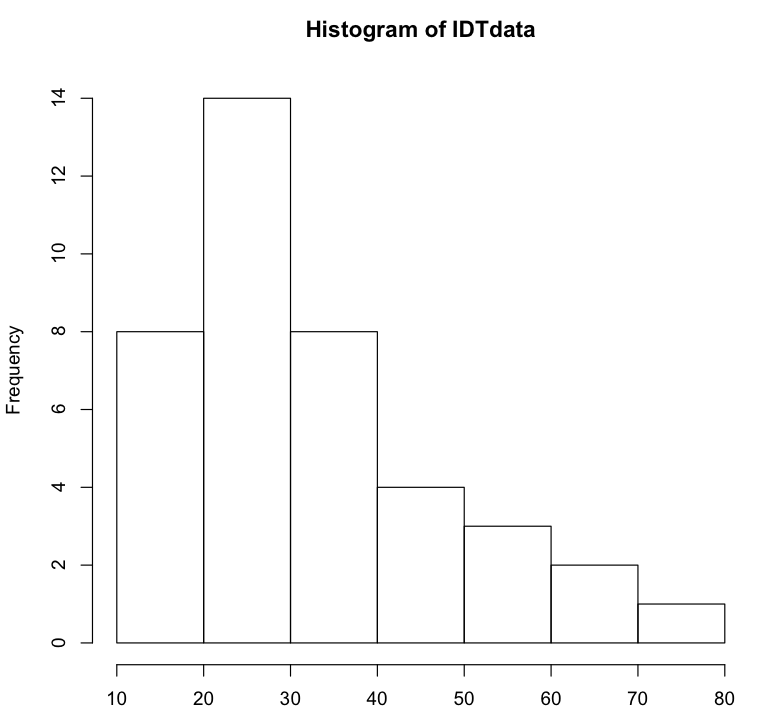
\includegraphics[width=0.75\textwidth]{IDTdata.png}
		\caption{IDT Data Histogram}
		\label{fig:IDT_data_hist}
	\end{figure}
	
	\begin{figure}[!htb]
		\centering
		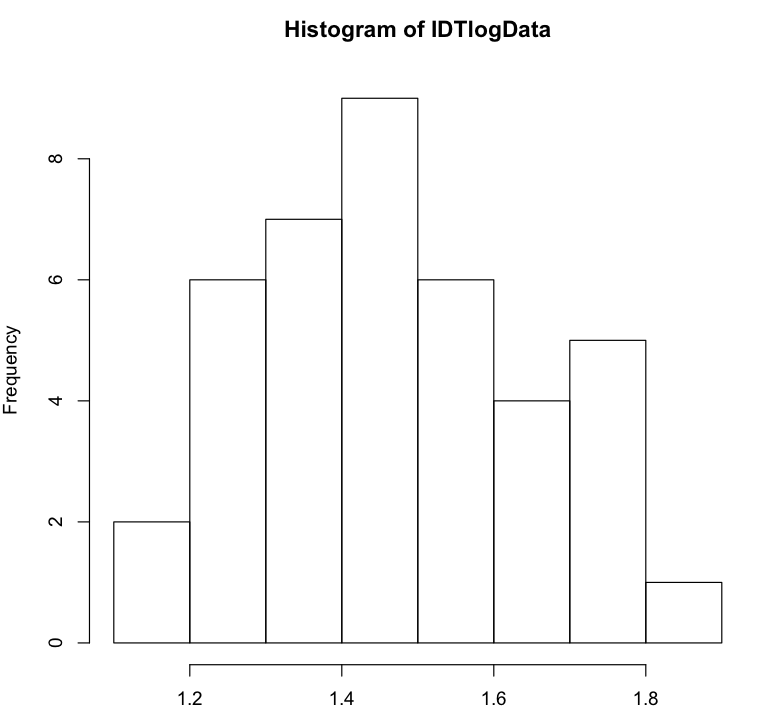
\includegraphics[width=0.75\textwidth]{IDTlogData.png}
		\caption{IDT Logarithmic Data Histogram}
		\label{fig:IDT_log_data_hist}
	\end{figure}
	
	There is a difference between the two graphs. The logarithmic one has just one more bar 
	representing data. This is mainly because of the data that the \texttt{hist()} function decided to 
	show. If we had showed all data and chosen smaller breaks than R, then we should have seen 
	basically the same histogram.

\clearpage
\section*{Problem 11}
\addcontentsline{toc}{section}{Eleventh Problem}

	A mail-order computer business has six telephone lines. Let x denote the number of lines in use 
	at a specified time. Suppose the mass function of x is given by \\
	
	\noindent p(0) = 0.10, \tab{p(1) = 0.15,} \tab{p(2) = 0.20,} \tab{p(3) = 0.25,} \\
	p(4) = 0.20, \tab{p(5) = ????,} \tab{p(6) =????.} \\
	
	\noindent (a) In the long run, what proportion of the time will at most three lines be in use? \\
	(b) In the long run, what proportion of the time will at least five lines be in use? \\
	(c) In the long run, what proportion of the time will between two and four lines, 
	inclusive, be in use? \\
	(d) In the long run, what proportion of the time will at least four lines NOT be in use?
	
	\paragraph{Answer to a}
	In order to solve this problem, we were already given all the data we need and all we have to do 
	is sum up the given proportions for under and including 3 telephone lines. In this case, the 
	answer is $P(x \le 3) = p(0) + p(1) + p(2) + p(3) = 0.10 + 0.15 + 0.20 + 0.25 = 0.7$.
	
	\paragraph{Answer to b}
	The way to solve this problem in nearly the same as the previous way except we are summing 
	together $p(5)$ and $p(6)$. We don't know what these values are, but it's easy to find out what 
	the two of them summed together are. The answer is $P(x \ge 5) = 1 - P(x \le 4) = 1 - (P(x \le 3) 
	+ P(4)) = 1 - (0.70 + 0.20) = 0.10$.
	
	\paragraph{Answer to c}
	The way to solve this problem is almost exactly the same as problem a, except this time we are 
	summing up $p(2)$, $p(3)$, and $p(4)$. The answer is $P(2 \le x \le 4) = p(2) + p(3) + p(4) = 
	0.20 + 0.25 + 0.20 = 0.65$.
	
	\paragraph{Answer to d}
	When answering this question, we have to think about which proportions we have to sum up so 
	we have to think about the way that this problem is worded. When saying that at least four lines 
	are not in use, then that means that, since there are only 6 lines, at most 2 lines are in use. The 
	answer to this question is $P(x \le 2) = p(0) + p(1) + p(2) = 0.10 + 0.15 + 0.20 = 0.45$.
		
\clearpage
\section*{Problem 12}
\addcontentsline{toc}{section}{Twelfth Problem}
	
	Suppose the density function for x is given by the normal distribution with parameters $\mu$, 
	$\sigma$.
	
	\begin{displaymath}
		f(x) = \frac{1}{\sqrt{2\pi\sigma^2}} e^{-\frac{1}{2}\left(\frac{x - \mu}{\sigma}\right)^2}
	\end{displaymath}
	
	\noindent (a) Compute the density function $ f(z) $ for $ z = \frac{x - \mu}{\sigma} $. \\

	\noindent (Hint: Recall that $ f(z) $ must satisfy $\int_{-\infty}^{\infty} f(z) dz = 1$. So start with 
	$\int_{-\infty}^{\infty} f(x) dx = 1 $ with $ f(x) $ as above, then make the substitution so it looks
	like $\int_{-\infty}^{\infty} f(z) dz = 1$. The new integrand after the substitution is the density for 
	the variable z.) \\

	\noindent (b) From the form of $f(z)$, read off its $\mu$ and $\sigma$ parameters.
	
	\paragraph{Answer to a}
	Understanding this question was a little difficult at first. When we substitute $z$ in for $x$ in the 
	standard distribution equation given above, then end up with the standard normal distribution 
	where $\mu = 0$ and $\sigma = 1$. In this case, the answer is:
	\begin{displaymath}
		f(z) = \frac{1}{\sqrt{2\pi (1^2)}} e^{-\frac{1}{2}\left(\frac{z - 0}{1}\right)^2}
	\end{displaymath}
	
	\paragraph{Answer to b}
	According to the equation found in the previous part of this problem, $\mu = 0$ and $\sigma = 
	1$.
	
\vspace{5.0\baselineskip}
\section*{Lab 1 Printouts}
\addcontentsline{toc}{section}{Lab 1 Prinouts}

Attached are the two printouts required for Lab 1.

\clearpage
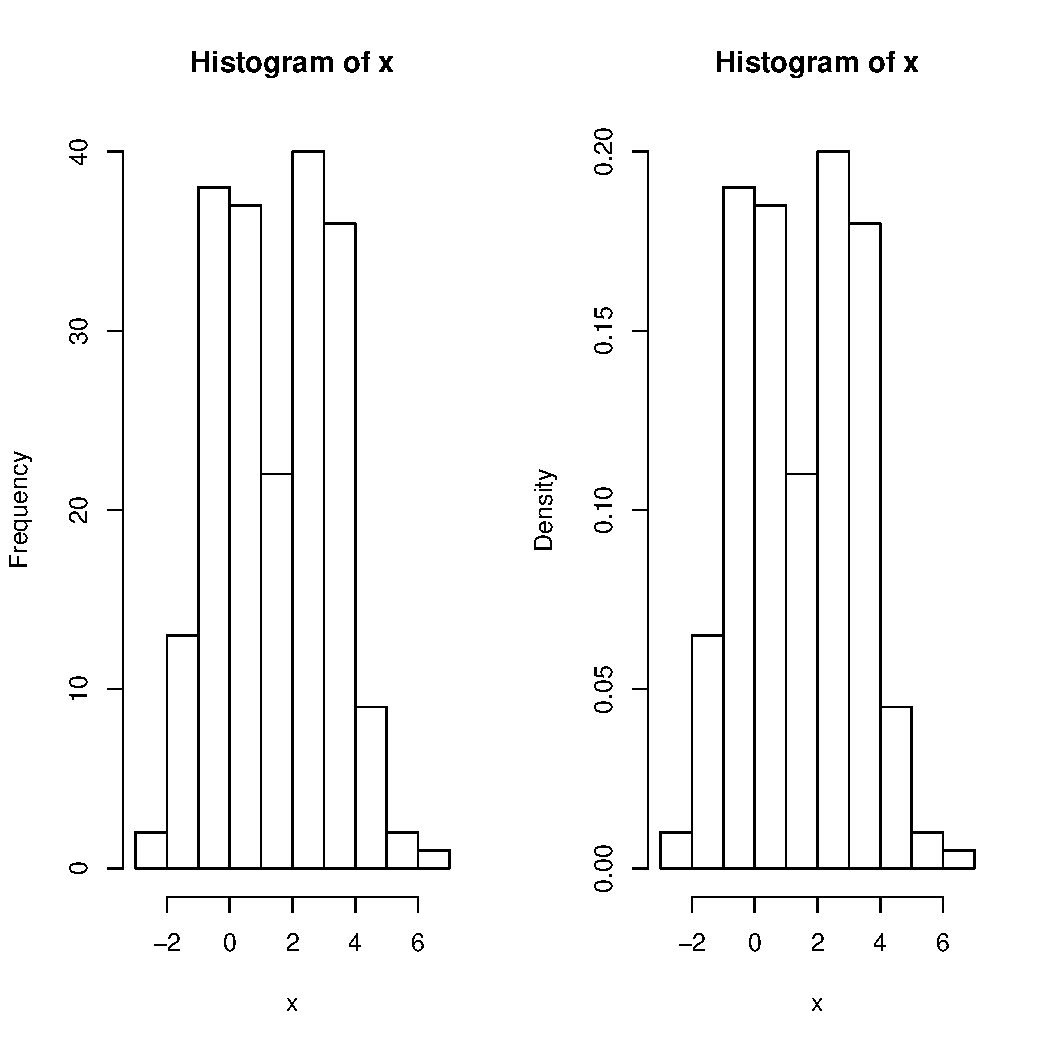
\includepdf[pages={1}]{hello.pdf}
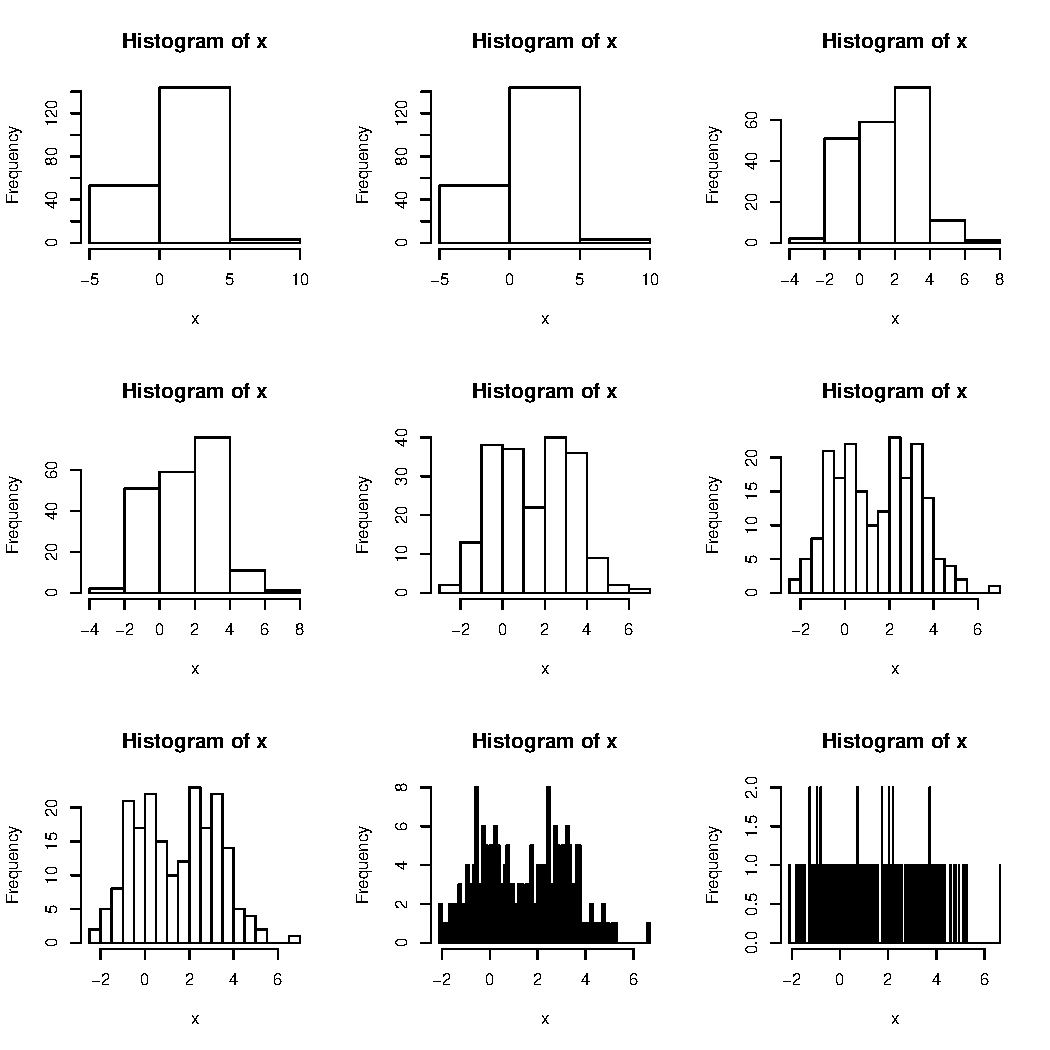
\includepdf[pages={1}]{hist_data.pdf}
	
\end{document}